\documentclass[a4paper,10pt,uplatex]{jsarticle}


% 数式
\usepackage{amsmath,amssymb,amsthm,bm}
\usepackage{mathtools}
\mathtoolsset{showonlyrefs}
\usepackage{physics}
\usepackage{siunitx}
\usepackage[thicklines]{cancel}
\usepackage{comment}
\usepackage{graphicx}
\usepackage[dvipdfmx]{color}
\usepackage{here}
\usepackage{tikz}

\newcommand{\rot}{\mathrm{rot}\;}
\renewcommand{\div}{\mathrm{div}\;}
\renewcommand{\grad}{\mathrm{grad}\;}
\newcommand{\E}{\vb*{E}}
\newcommand{\B}{\vb*{B}}
\newcommand{\D}{\vb*{D}}
\renewcommand{\P}{\vb*{P}}
\renewcommand{\H}{\vb*{H}}
\newcommand{\A}{\vb*{A}}
\newcommand{\x}{\vb*{x}}
\renewcommand{\i}{\vb*{i}}
\newcommand{\n}{\vb*{n}}

\newcommand{\ds}{\displaystyle}

\begin{document}

\title{ベクトル解析}
\author{}
\date{\today}
\maketitle

\section{直交曲線座標系でのベクトル演算子}
直交曲線座標系を$(t_1, t_2, t_3)$ととる(例えば極座標$(r,\theta,\phi$)など).$t_i$の方向に距離$ds_i$だけ移動すると,座標は$t_i+dt_i$になる.逆に,座標$t_i + dt_i$になるには,距離$ds_i$だけ移動しなければならないとも言える.このとき$dt_i$と$ds_i$の間には$ds_i = h_i dt_i$という関係が成り立つ.$h_i$は$t_j$の関数である.

\subsection{勾配(gradient)}
あるスカラー関数$f$について,ある点から,その点の周りで値が最も大きくなる方向はどちらかを知りたい.つまり,勾配(gradient)を求めたい.そのためには,各方向について,少しだけ移動してみて,その変化具合を調べればよい.デカルト座標系では,$x$方向ならば$dx$移動して$f(x+dx)$の値を調べてくれば,$x$方向の傾きがわかる.一般の直交曲線座標系では$t_i$方向に移動して$f(t_i+dt_i)$を調べるには,$ds_i$だけ移動する必要がある.したがって勾配は
\begin{equation}
    \pdv{s_i} = \frac{1}{h_i}\pdv{t_i}
\end{equation}
となる.

静電場と静電ポテンシャルの関係式
\begin{equation}
    \E(\x) = -\grad \phi(\x)
\end{equation}
は,電場は,静電ポテンシャルが最もはやく減る方向を向いていることを意味している.

\subsection{発散(divergence)}
ベクトル関数$f$について,ベクトルは大きさを持った矢印で,流れのようなイメージを持つ.流れというからには発生源があるだろうから,その「湧き出し」というものを調べたい.これが発散(divergence)である.そのためには,微小体積の領域を考えて,その領域での流出量を調べればよい.流出量が正ならば,その領域には流れの発生源があることになる.\footnote{ここに図を挿入}
\begin{align}
    &f_1(t+dt_1, t_2, t_3) ds_2' ds_3' - f_1(t_1, t_2, t_3) ds_2 ds_3 \\
    &\quad = \left(f_1 + \pdv{f_1}{t_1}dt_1\right)\left(h_2+\pdv{h_2}{t_1}dt_1\right)dt_2\left(h_3+\pdv{h_3}{t_1}dt_1\right)dt_3 - f_1h_2h_3dt_2dt_3 \\
    &\quad = \left(f_1h_2\pdv{h_3}{t_1}dt_1 + f_1h_3\pdv{h_2}{t_1}dt_1 + h_2h_3\pdv{f_1}{t_1}dt_1\right)dt_2dt_3 \\
    &\quad = \pdv{t_1}(f_1h_2h_3)dt_1dt_2dt_3
\end{align}
途中の計算で4次以上の項は無視した.同様にして$t_2$方向,$t_3$方向についても流出量を計算すると,全体で合計は
\begin{equation}
    dt_1dt_2dt_3 \sum_i \pdv{t_i}\left(\frac{h_1h_2h_3f_i}{h_i}\right)
\end{equation}
となる.ところで,微小体積は($h_i$が$t_j$によるので)座標によって変わってしまう.つまり上の結果には領域のとり方の影響が残っている.微小体積$dV = ds_1ds_2ds_3$で割ることで,単位体積あたりの流出量となって,これは領域のとり方によらない値となる.これが発散である:
\begin{equation}
    \div \vb*{f} = \frac{1}{h_1h_2h_3} \sum_i \pdv{t_i}\left(\frac{h_1h_2h_3f_i}{h_i}\right)
\end{equation}

電場と電荷密度の関係式
\begin{equation}
    \div \E(\x,t) = \frac{\rho(\x,t)}{\varepsilon_0}
\end{equation}
は,電場は電荷から湧き出てくる(発生する)ことを意味している.

\subsection{回転(rotation)}
\begin{center}
\tikzset{every picture/.style={line width=0.75pt}} %set default line width to 0.75pt        

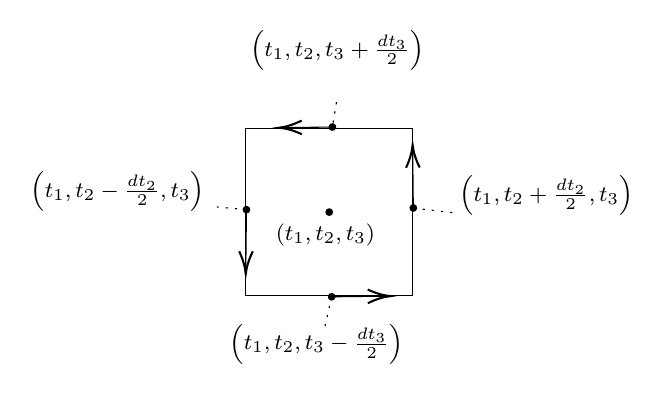
\begin{tikzpicture}[x=0.75pt,y=0.75pt,yscale=-1,xscale=1]
%uncomment if require: \path (0,300); %set diagram left start at 0, and has height of 300

%Shape: Rectangle [id:dp5664680057342357] 
\draw   (139.33,100.33) -- (219.67,100.33) -- (219.67,181) -- (139.33,181) -- cycle ;
%Straight Lines [id:da8098348518235821] 
\draw    (181,99.67) -- (157.33,99.97) ;
\draw [shift={(155.33,100)}, rotate = 359.26] [color={rgb, 255:red, 0; green, 0; blue, 0 }  ][line width=0.75]    (10.93,-3.29) .. controls (6.95,-1.4) and (3.31,-0.3) .. (0,0) .. controls (3.31,0.3) and (6.95,1.4) .. (10.93,3.29)   ;
%Straight Lines [id:da6303992678375832] 
\draw    (180.67,181.47) -- (207,181.16) ;
\draw [shift={(209,181.13)}, rotate = 179.33] [color={rgb, 255:red, 0; green, 0; blue, 0 }  ][line width=0.75]    (10.93,-3.29) .. controls (6.95,-1.4) and (3.31,-0.3) .. (0,0) .. controls (3.31,0.3) and (6.95,1.4) .. (10.93,3.29)   ;
%Straight Lines [id:da9863714267047494] 
\draw    (220,138.67) -- (219.69,110.33) ;
\draw [shift={(219.67,108.33)}, rotate = 89.37] [color={rgb, 255:red, 0; green, 0; blue, 0 }  ][line width=0.75]    (10.93,-3.29) .. controls (6.95,-1.4) and (3.31,-0.3) .. (0,0) .. controls (3.31,0.3) and (6.95,1.4) .. (10.93,3.29)   ;
%Straight Lines [id:da7515251565664738] 
\draw    (139.6,139.47) -- (139.29,168.47) ;
\draw [shift={(139.27,170.47)}, rotate = 270.62] [color={rgb, 255:red, 0; green, 0; blue, 0 }  ][line width=0.75]    (10.93,-3.29) .. controls (6.95,-1.4) and (3.31,-0.3) .. (0,0) .. controls (3.31,0.3) and (6.95,1.4) .. (10.93,3.29)   ;
%Straight Lines [id:da5168038312878571] 
\draw  [dash pattern={on 0.84pt off 2.51pt}]  (183,87.67) -- (181,99.67) ;
\draw [shift={(181,99.67)}, rotate = 99.46] [color={rgb, 255:red, 0; green, 0; blue, 0 }  ][fill={rgb, 255:red, 0; green, 0; blue, 0 }  ][line width=0.75]      (0, 0) circle [x radius= 1.34, y radius= 1.34]   ;
%Straight Lines [id:da4820220338164427] 
\draw  [dash pattern={on 0.84pt off 2.51pt}]  (220,138.67) -- (239.4,141) ;
\draw [shift={(220,138.67)}, rotate = 6.86] [color={rgb, 255:red, 0; green, 0; blue, 0 }  ][fill={rgb, 255:red, 0; green, 0; blue, 0 }  ][line width=0.75]      (0, 0) circle [x radius= 1.34, y radius= 1.34]   ;
%Straight Lines [id:da8115295364026136] 
\draw  [dash pattern={on 0.84pt off 2.51pt}]  (180.67,181.47) -- (177.4,195.8) ;
\draw [shift={(180.67,181.47)}, rotate = 102.84] [color={rgb, 255:red, 0; green, 0; blue, 0 }  ][fill={rgb, 255:red, 0; green, 0; blue, 0 }  ][line width=0.75]      (0, 0) circle [x radius= 1.34, y radius= 1.34]   ;
%Straight Lines [id:da4092663572232891] 
\draw  [dash pattern={on 0.84pt off 2.51pt}]  (139.6,139.47) -- (125.4,138.2) ;
\draw [shift={(139.6,139.47)}, rotate = 185.1] [color={rgb, 255:red, 0; green, 0; blue, 0 }  ][fill={rgb, 255:red, 0; green, 0; blue, 0 }  ][line width=0.75]      (0, 0) circle [x radius= 1.34, y radius= 1.34]   ;
%Straight Lines [id:da74678777657573] 
\draw    (179.5,140.67) ;
\draw [shift={(179.5,140.67)}, rotate = 0] [color={rgb, 255:red, 0; green, 0; blue, 0 }  ][fill={rgb, 255:red, 0; green, 0; blue, 0 }  ][line width=0.75]      (0, 0) circle [x radius= 1.34, y radius= 1.34]   ;

% Text Node
\draw (140.17,52.07) node [anchor=north west][inner sep=0.75pt]  [font=\footnotesize]  {$\left( t_{1} ,t_{2} ,t_{3} +\frac{dt_{3}}{2}\right)$};
% Text Node
\draw (130.37,193.37) node [anchor=north west][inner sep=0.75pt]  [font=\footnotesize]  {$\left( t_{1} ,t_{2} ,t_{3} -\frac{dt_{3}}{2}\right)$};
% Text Node
\draw (240.97,121.87) node [anchor=north west][inner sep=0.75pt]  [font=\footnotesize]  {$\left( t_{1} ,t_{2} +\frac{dt_{2}}{2} ,t_{3}\right)$};
% Text Node
\draw (34.47,119.87) node [anchor=north west][inner sep=0.75pt]  [font=\footnotesize]  {$\left( t_{1} ,t_{2} -\frac{dt_{2}}{2} ,t_{3}\right)$};
% Text Node
\draw (152.47,145.2) node [anchor=north west][inner sep=0.75pt]  [font=\footnotesize]  {$( t_{1} ,t_{2} ,t_{3})$};


\end{tikzpicture}
\end{center}


ベクトル関数$\vb*{f}$について,今度は流れの「渦っぽさ」というものを調べる.これが回転(rotation)である.渦というのは2次元的なイメージなので,3次元空間ならばそれは3方向あることになる.したがって回転はベクトル量となる.まず$t_1$方向に直交する面について,中心を$(t_1,t_2,t_3)$として,$t_2, t_3$軸方向と平行な辺を持つ以下のような四角形を考える.$t_2$軸に平行な方向について,
\begin{align}
    &f_2(t_1,t_2,t_3-\frac{dt_3}{2})ds_2 - f_2(t_1,t_2,t_3+\frac{dt_3}{2})ds_2'  \\
    &= dt_2\left[\left(f_2 - \frac{dt_3}{2}\pdv{f_2}{t_3}\right)\left(h_2 - \frac{dt_3}{2}\pdv{h_2}{t_3}\right) - \left(f_2 + \frac{dt_3}{2}\pdv{f_2}{t_3}\right)\left(h_2 + \frac{dt_3}{2}\pdv{h_2}{t_3}\right)\right] \\
    &= dt_2\left(-f_2\pdv{h_2}{t_3}dt_3 - \pdv{f_2}{t_3}h_2 dt_3\right) \\
    &= -dt_2dt_3\pdv{t_3}(f_2h_2)
\end{align}
である.$t_3$軸に平行な方向は,
\begin{align}
    &f_3\left(t_1,t_2+\frac{dt_2}{2},t_3\right)ds_3' - f_3\left(t_1,t_2-\frac{dt_2}{2},t_3\right)ds_3 \\
    &= dt_3\left[\left(f_3 + \frac{dt_2}{2}\pdv{f_3}{t_2}\right)\left(h_3+\frac{dt_2}{2}\pdv{h_3}{t_2}\right) - \left(f_3 - \frac{dt_2}{2}\pdv{f_3}{t_2}\right)\left(h_3-\frac{dt_2}{2}\pdv{h_3}{t_2}\right)\right] \\
    &= dt_2dt_3\left(f_3\pdv{h_3}{t_2} + \pdv{f_3}{t_2}h_3\right) \\
    &= dt_2dt_3\pdv{t_2}(f_3h_3)
\end{align}
となる.この和をとると
\begin{equation}
    dt_2dt_3\left(\pdv{t_2}(f_3h_3) - \pdv{t_3}(f_2h_2)\right)
\end{equation}
となるが,これにはまだ四角形の微小面積の影響が残っている.四角形の各辺の長さはばらばらなので,$ds_2$と$ds_2'$の平均,$ds_3$と$ds_3'$の平均を2辺とする長方形として面積を計算すると,$h_2h_3dt_2dt_3$となる.したがって求めたかった$\rot \vb*{f}$の第1成分は
\begin{equation}
    \frac{1}{h_2h_3}\left(\pdv{t_2}(f_3h_3) - \pdv{t_3}(f_2h_2)\right)
\end{equation}
となる.他の2成分についても同様で,一般化すると
\begin{equation}
    (\rot \vb*{f})_i = \frac{h_i}{h_1h_2h_3}\varepsilon_{ijk}\pdv{t_j}(f_kh_k)
\end{equation}

\subsection{Laplacian}
これまで考えてきた勾配と発散を組み合わせた演算子$\Delta = \div \grad$がLaplacianである.この表記だとスカラー関数にしか作用できないが,実際にはベクトル関数にも作用できる.ベクトルの各要素に対して作用する.

まずはスカラー関数に作用することを考える.勾配の発散である.勾配というのは,どちらに進めば最も値が大きく変化するかを表すものだった.したがって,勾配のベクトル場を考えると,極大値を取るところではベクトルが一点に集まってくるようになっている.逆に,極小値を取るところでは,ベクトルが一点から外に出ていくようになっている.この発散を考えると,流出量を考えるのだから,極大値では負,極小値では正をとる.一方で,勾配が一定の方向を向いている場合や,一方向だけ見ると流入/出過多でも,他の方向の流出/入も考慮するとちょうどキャンセルしあっているような場合にも0になる.
ベクトル関数に作用するときは,各成分に対して,スカラー関数と同じように作用するので,あまり違いはない.

このような考察から,スカラー関数に対するLaplacianは,「起伏」を表すようなものであるとイメージできる.その点が山にあたるなら負の値を,谷にあたるなら正の値を,平らな台地なら0をとる.そして,ベクトル関数に対しては,関数の成分の「起伏」を成分にもつベクトルを得る\footnote{これが何を意味するのかはよくわからない}.

Laplacianの公式は,上で求めた勾配,発散の公式を使えばすぐに出てくる.
\begin{equation}
    \Delta f = \div \grad f = \frac{1}{h_1h_2h_3} \sum_i \pdv{t_i}\left(\frac{h_1h_2h_3}{h_i^2}\pdv{f}{t_i}\right)
\end{equation}

Poisson方程式
\begin{equation}
    \Delta \phi(\x) = -\frac{1}{\varepsilon_0}\rho(\x)
\end{equation}
は,電荷によって静電ポテンシャルは起伏を持つことを意味している.正電荷ならば山に,負電荷ならば谷になる.電場は,このようにしてできた静電ポテンシャルの起伏を,最も急激に下るような方向を向いている.

\section{積分計算}

\subsection{面積分}
基本となる座標系はデカルト座標$(x,y,z)$である.線分の長さは$\sqrt{dx^2+dy^2+dz^2}$のように表される.この座標系上の曲面を2つのパラメータ$s,t$を使って$S:\vb*{r}(s,t)$と表す.このとき,曲面には$s$,$t$による,歪んでいてもよい目盛り(網目)が張り巡らされる.曲面上の点は$(s,t)$を指定すれば一意に定まるからである.今$(s,t)$にいるとき,微小な距離だけ進んで$(s+ds,t)$に行くにはどちらの方向にどれだけ進めば良いのだろうか.\footnote{この答えは$ds$ではないことに気をつけねばならない.なぜなら距離は基本となる座標系(デカルト座標系)によって定義されているものだからだ.}
この答えは
\begin{equation}
    \vb*{r}(s+ds,t) - \vb*{r}(s,t) \to \pdv{\vb*{r}(s,t)}{s} ds
\end{equation}
となる.$t$についても同様で,$(s,t)$から$(s,t+dt)$に行くには$(\partial\vb*{r}(s,t)/\partial t)dt$移動すればよい.ところで$(s,t)$における面の法線ベクトルは,この点から面上でどの方向に進むベクトルとも直交するベクトルのことである.したがって法線ベクトルの方向は,上で求めた微小移動を表す2つのベクトルの外積として表せる(向きは2方向ありえる).また,この曲線上の微小面積$dS$は,$(s,t)$と$(s+ds,t+dt)$の間の平行四辺形の面積のこと.同様に外積を使えば
\begin{equation}
    dS = \left|\pdv{\vb*{r}(s,t)}{s} \times \pdv{\vb*{r}(s,t)}{t}\right|dsdt
\end{equation}
と書ける.したがって,曲線上の面積分は,まずスカラー場について
\begin{equation}
    \iint_S f(\vb*{r}) \dd{S} = \iint_D f(\vb*{r}(s,t)) \left|\pdv{\vb*{r}}{s} \times \pdv{\vb*{r}}{t}\right|\dd{s}\dd{t}
\end{equation}
となる.ここで$D$は$s,t$の取りうる領域.ベクトル場については
\begin{equation}
    \iint_S \vb*{f}(\vb*{r}) \cdot \vb*{n} \dd{S} = \iint_D \vb*{f}(\vb*{r}(s,t)) \cdot \left( \pdv{\vb*{r}}{s} \times \pdv{\vb*{r}}{t}\right) \dd{s}\dd{t}
\end{equation}
となる.$\vb*{n}$は法線ベクトルで,ここでは
\begin{equation}
    \vb*{n} = \pdv{\vb*{r}}{s} \times \pdv{\vb*{r}}{t}
\end{equation}
ととっている.法線ベクトルのとりかたによって,符号の異なる2つの結果があり得る.

\subsection{体積積分}
ある領域の内部をパラメータ$s,t,u$を使って$\vb*{r}(s,t,u)$と表す.面積分のときと同様にして,領域にこれらによる目盛りが張り巡らされる.このとき微小体積要素は,
\begin{align}
    dV &= \left| \left(\pdv{\vb*{r}}{s} \times \pdv{\vb*{r}}{t}\right) \cdot \pdv{\vb*{r}}{u} \right| dsdtdu \\
    &= \mqty| \ds \pdv{\vb*{r}}{s} \; \pdv{\vb*{r}}{t} \; \pdv{\vb*{r}}{u} | dsdtdu
\end{align}
である.最後の式は行列式だが,ヤコビアンとも呼ばれる.行列式の性質として,転置しても結果が変わらない.
このとき体積積分は
\begin{equation}
    \iiint_D f(\vb*{r}) dV = \iiint_D f(\vb*{r}(s,t,u)) \mqty| \ds \pdv{\vb*{r}}{s} \; \pdv{\vb*{r}}{t} \; \pdv{\vb*{r}}{u} | \dd{s}\dd{t}\dd{u}
\end{equation}
となる.

\section{直交曲線座標系の基底}
直交曲線座標系を$(t_1, t_2, t_3)$ととる(例えば極座標$(r,\theta,\phi$)など).空間の各点は,この3つのパラメータと一対一に対応する.さて,この座標系がデカルト座標系$(x,y,z)$だったら,$(x,y,z)$から例えば$(x+dx,y,z)$に行くには,$x$軸に沿って$dx$だけ移動すれば良い.この方向はどの点についても変わらず一定だ.しかし,曲線座標系だとこの方向が各点で異なる.例として極座標を考えると,点P$(r,\theta,\phi)$からP'$(r+dr,\theta,\phi)$に行くには,原点Oから$\va{OP}$の方向に$dr$だけ進まなければいけない.この方向はPの位置によっていろいろと変わる.したがって,デカルト座標系を考えていたときは空間は一様で,どこで基底を考えても不自由することはなかったが,一般の直交曲線座標系を考えるときは,どの点を基準にして基底とするかを考えなければいけない\footnote{例えば極座標をとるとき,原点では基底を取るような特別な方向がない}.

\end{document}